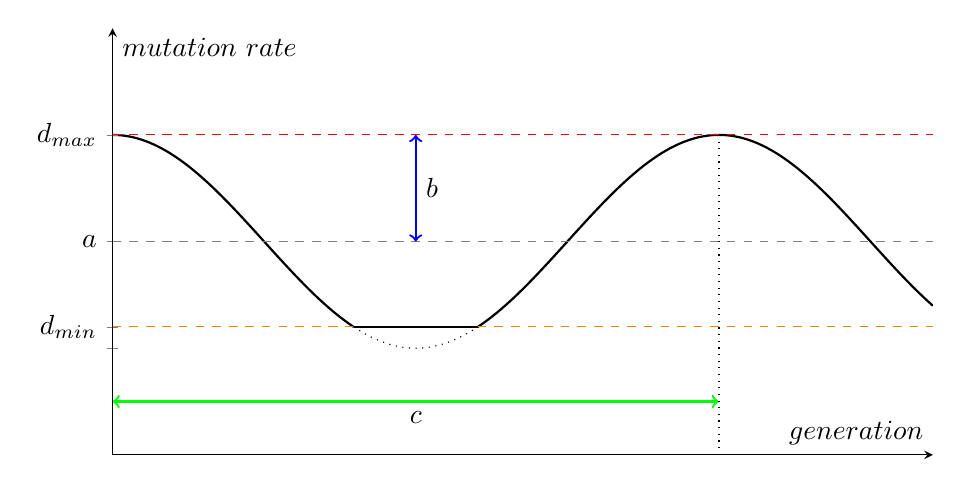
\begin{tikzpicture}
    \begin{axis}[
        axis lines=middle, % Draw axes
        xlabel={$generation$}, % Label x-axis
        ylabel={$mutation$ $rate$}, % Label y-axis
        domain=0:8.5, % Domain for cosine wave (1.5 wavelength)
        xmin=0, xmax=8.5, % Adjust x-axis range
        ymin=0, ymax=4.0, % Adjust y-axis range
        xtick=\empty, % Remove automatic x-ticks
        ytick={1, 1.2, 2, 3}, % Set custom y-ticks
        yticklabels={, $d_{min}$, $a$, $d_{max}$}, % Custom labels for y-ticks
        samples=100, % Number of samples for smooth curve
        width=12cm, % Width of the plot
        height=7cm, % Height of the plot
        axis on top % ensures that the axis are rendered on top
        % smooth, % Smooth curves
    ]

        % Cosine wave with "dent"
        \addplot[black, thick, domain=0:2.49809] {cos(deg(x)) + 2};
        \addplot[black, dotted, domain=2.49809:3.78509] {cos(deg(x)) + 2};
        \addplot[black, thick, domain=3.78509:8.5] {cos(deg(x)) + 2};

        \addplot[black, thick, domain=2.49809:3.78509] {1.2};

        % Draw dashed lines for d_max and d_min
        \addplot[red, dashed] {3};
        \addplot[orange, dashed, domain=0:2.49809] {1.2};
        \addplot[orange, dashed, domain=3.78509:8.5] {1.2};

        % Draw dashed lines for middle
        \addplot[gray, dashed] {2};

        % Mark amplitude
        \draw[<->, blue, thick]
            (axis cs:3.14159,2.0) -- (axis cs:3.14159,3.0)
            node[midway, right, black] {$b$};

        % Mark wavelength
        \draw[<->, green, thick]
            (axis cs:0,0.5) -- (axis cs:6.2832,0.5)
            node[midway, below, black] {$c$};

        \draw[-, dotted]
            (axis cs:6.2832,3.0) -- (axis cs:6.2832,0.0);

        % Add annotations for minima
        % \node[anchor=east] at (axis cs:1.0472, 0) {$d_{min}$};
        % \node[anchor=east] at (axis cs:3.14159, 0) {$d_{min}$};
        % \node[anchor=east] at (axis cs:5.236, 0) {$d_{min}$};
    \end{axis}

\end{tikzpicture}
